\subsection*{a)}
	Using the law of mass action, we can say that the product of our majority and minority carrier concentrations (holes and electrons, respectively) is equal to the square of the intrinsic carrier concentration, $n_i$. Since $n_i^2 = N_C N_V \exp\left(\dfrac{-E_g}{k_B T}\right)$, $n_i$ has a value of $6.57 \times 10^{9} \textrm{ cm}^{-3}$ in silicon, at room temperature. This holds so long as the base region is large, and hence the emitter and collector can be ignored. Under an assignment amendment, the value of $n_i = 1.0 \times 10^{10}$ will be used.
	
	We can take the majority carrier concentration, $p_{p0}$, to be approximately $N_A = 10^9 \textrm{ cm}^{-3}$, and so our minority carrier concentration must be $n_{p0} = \dfrac{n_i^2}{p_{p0}} = \dfrac{10^{20}}{10^{19}} = 10 \textrm{ cm}^{-3}$.
\subsection*{b)}
	The minority carrier concentration can be expressed as
	$$\Delta n(x) = 
	\Delta n_2 \frac{\sinh\left(\frac{W_B - x_b}{L_n}\right)}{\sinh\left(\frac{W_B}{L_n}\right)} + 
	\Delta n_3 \frac{\sinh\left(\frac{x_b}{L_n}\right)}{\sinh\left(\frac{W_B}{L_n}\right)}
	$$	
	where
	\[
		\begin{aligned}
		\Delta n(x_b) &= n(x_b) - n_{p0} \\
		\Delta n_2  &= n(0) - n_{p0} \\
		\Delta n_3  &= n(W_B) - n_{p0} \\	
		\end{aligned}
	\]
	
	If we treat the base-emitter and base-collector regions as two separate diodes, we can define the minority carrier concentration at the interfaces of the transition regions from the base side as follows: \\
	
	\noindent For the base-emitter junction
	$$\Delta n(x_b = 0) = \Delta n_2 
			= \frac{n_i^2}{N_A}
			 \left(
				\exp{\left(
					\frac{- q V_{BE}}{k_B T}				
				\right)} - 1
			\right)
	$$
	For the base-collector junction
	$$\Delta n(x_b = W_B) = \Delta n_3
	= \frac{n_i^2}{N_A}
	\left(
		\exp{\left(
			\dfrac{q V_{BC}}{k_B T}				
		\right)} - 1
	\right)
	$$
	
\subsection*{c)}
	The plot shown in Figure \ref{fig::3c} depicts the minority carrier concentration in the base under cut-off conditions. This is clear as there is a large drop off in carrier concentration on the emitter side, which implies that carriers injected from the collector are not reaching the emitter, hence the transistors is "off".
	
	This scheme exhibits low recombination of minority carriers in the base, and our original equation can be approximated as
	\[
	\begin{aligned}
		\Delta n(x) &= \Delta n_2 \left(1 - \dfrac{x_b}{W_B}\right) +
		\Delta n_3 \left(\dfrac{x_b}{W_B}\right) \\
					&= 1
	\end{aligned}
	\]
	In this figure, this is depicted as an overlay, which exactly meets our simulated results.
	
	\begin{figure}[htbp!]
		\centering
		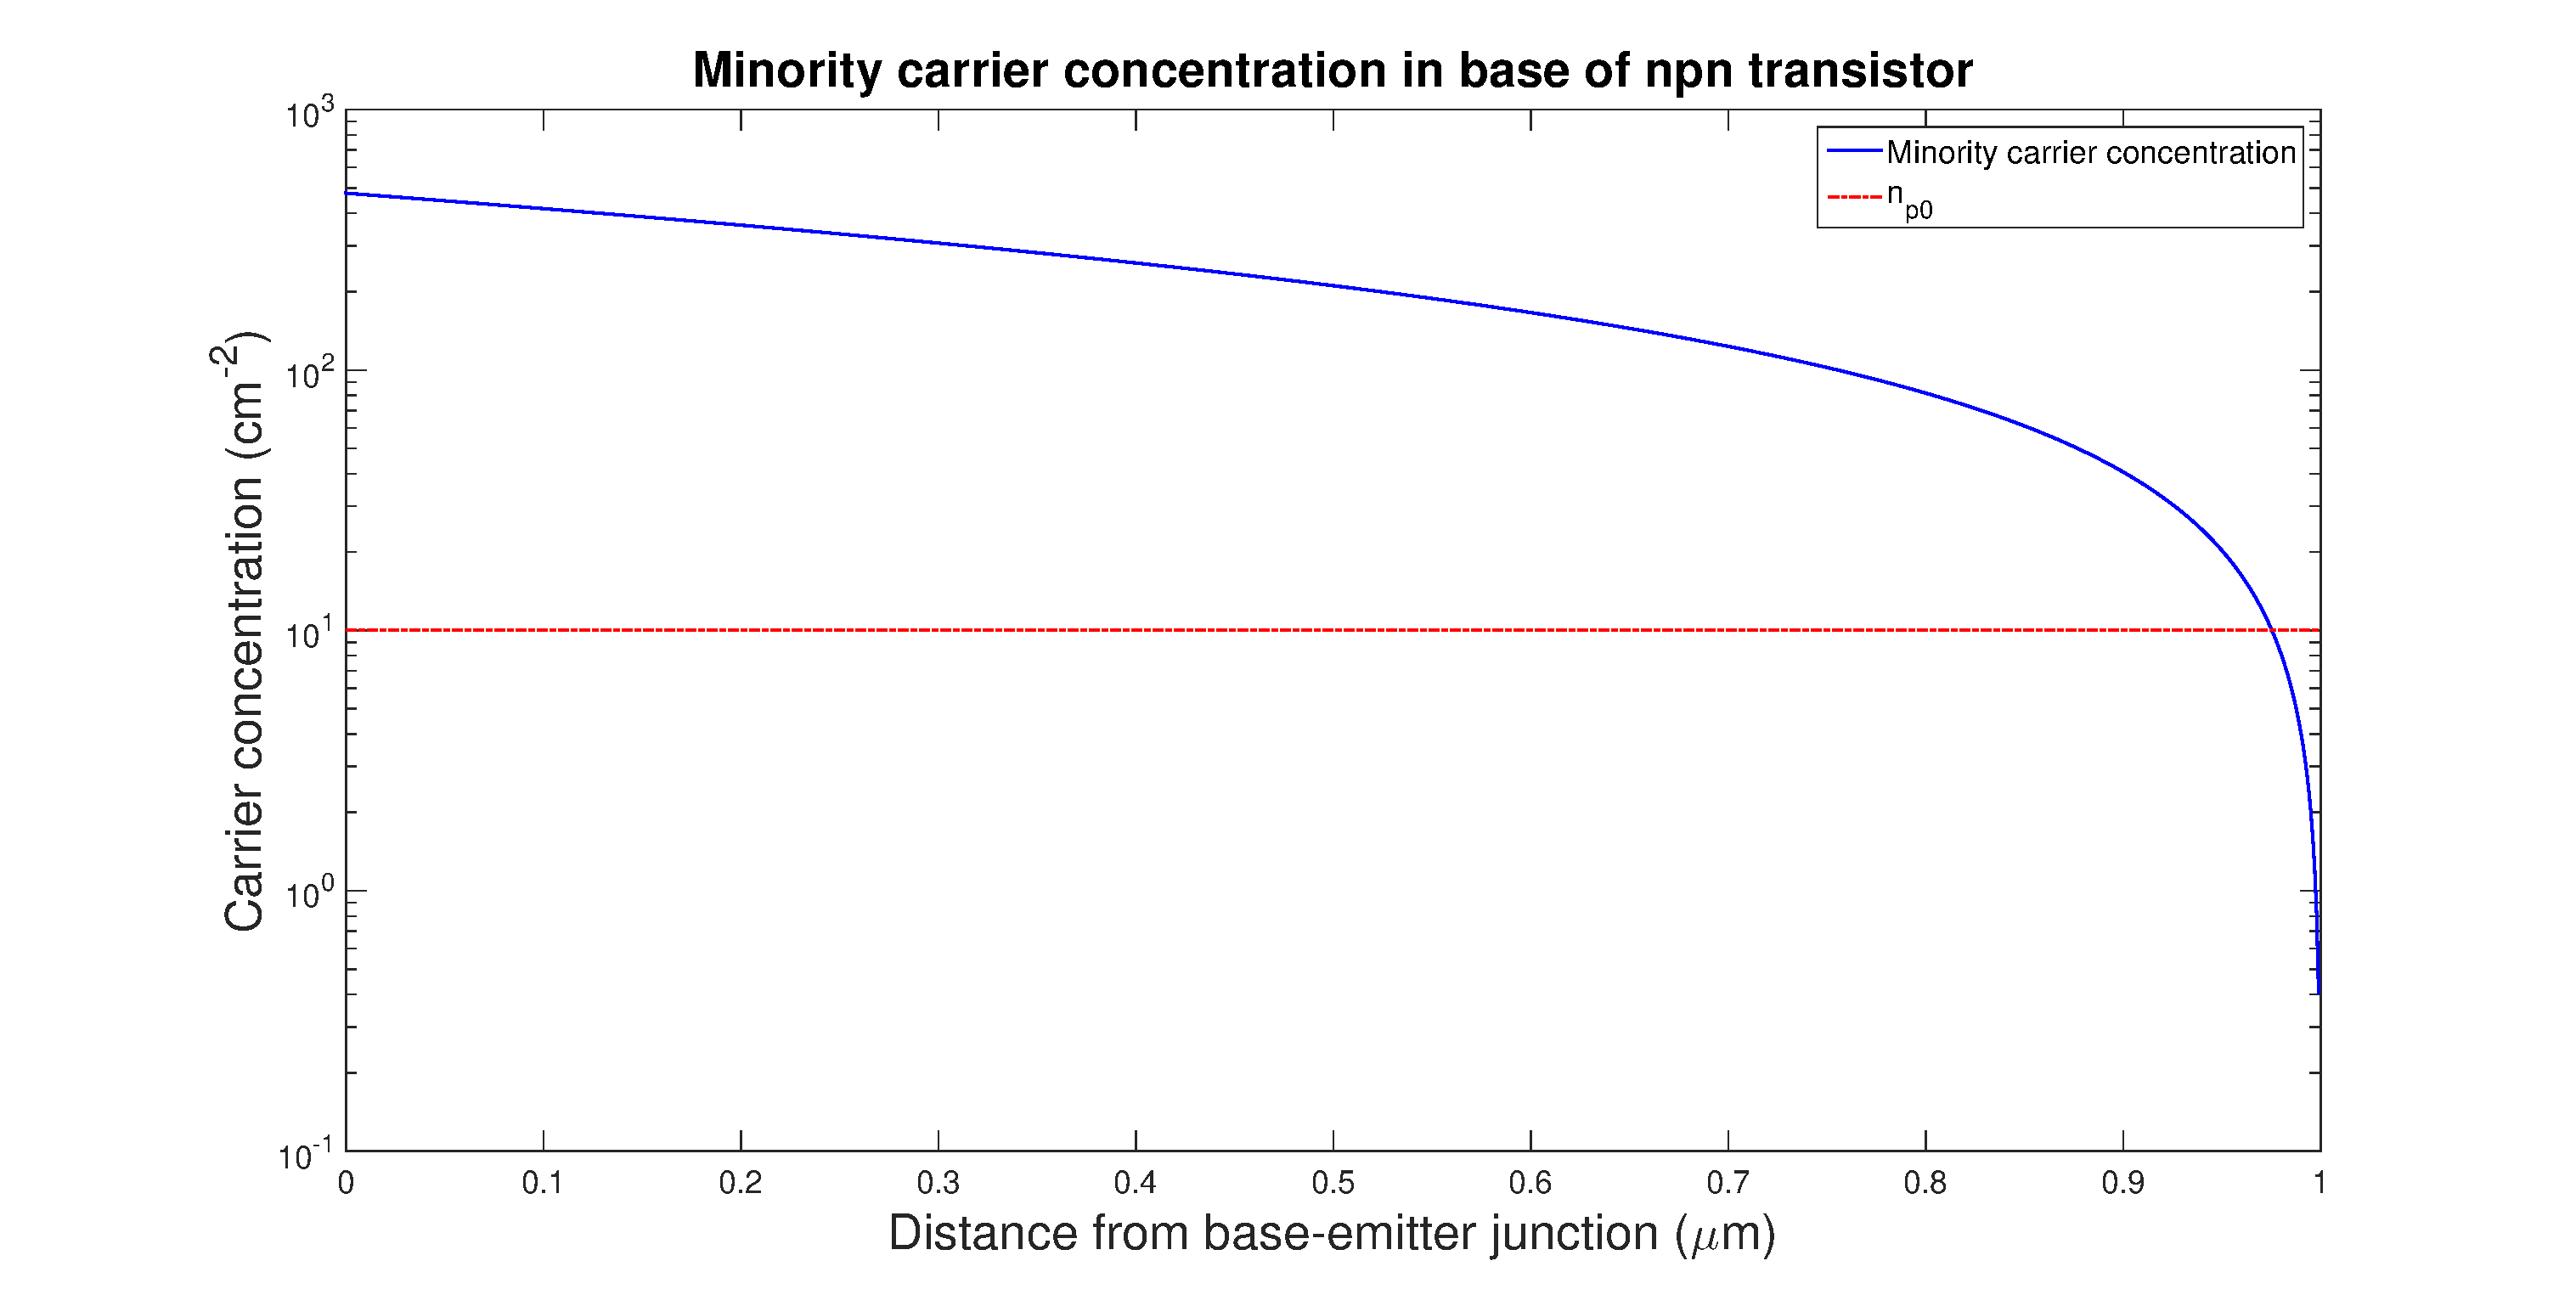
\includegraphics[width=0.8\textwidth]{./img/3c}
		\caption{Minority carrier concentration for a base width $W_B = 1 \mu m$.}
		\label{fig::3c}
	\end{figure}
\subsection*{d)}
	The plot shown in Figure \ref{fig::3c} shows the minority carrier concentration when the base is large compared to the diffusion length of the carrier. This scheme exhibits high recombination of minority carriers in the base, and our original equation can be approximated as
	\[
	\begin{aligned}
		\Delta n(x) &= \Delta n_2 \exp\left(\dfrac{-x_b}{L_n}\right) +					\Delta n_3 \exp\left(\dfrac{x_b-W_B}{L_n}\right) \\
					&= 1
	\end{aligned}
	\]
	In the figure, this is depicted as an overlay, which eclipses the original function showing that it is an accurate approximation.
	\begin{figure}[htbp!]
		\centering
		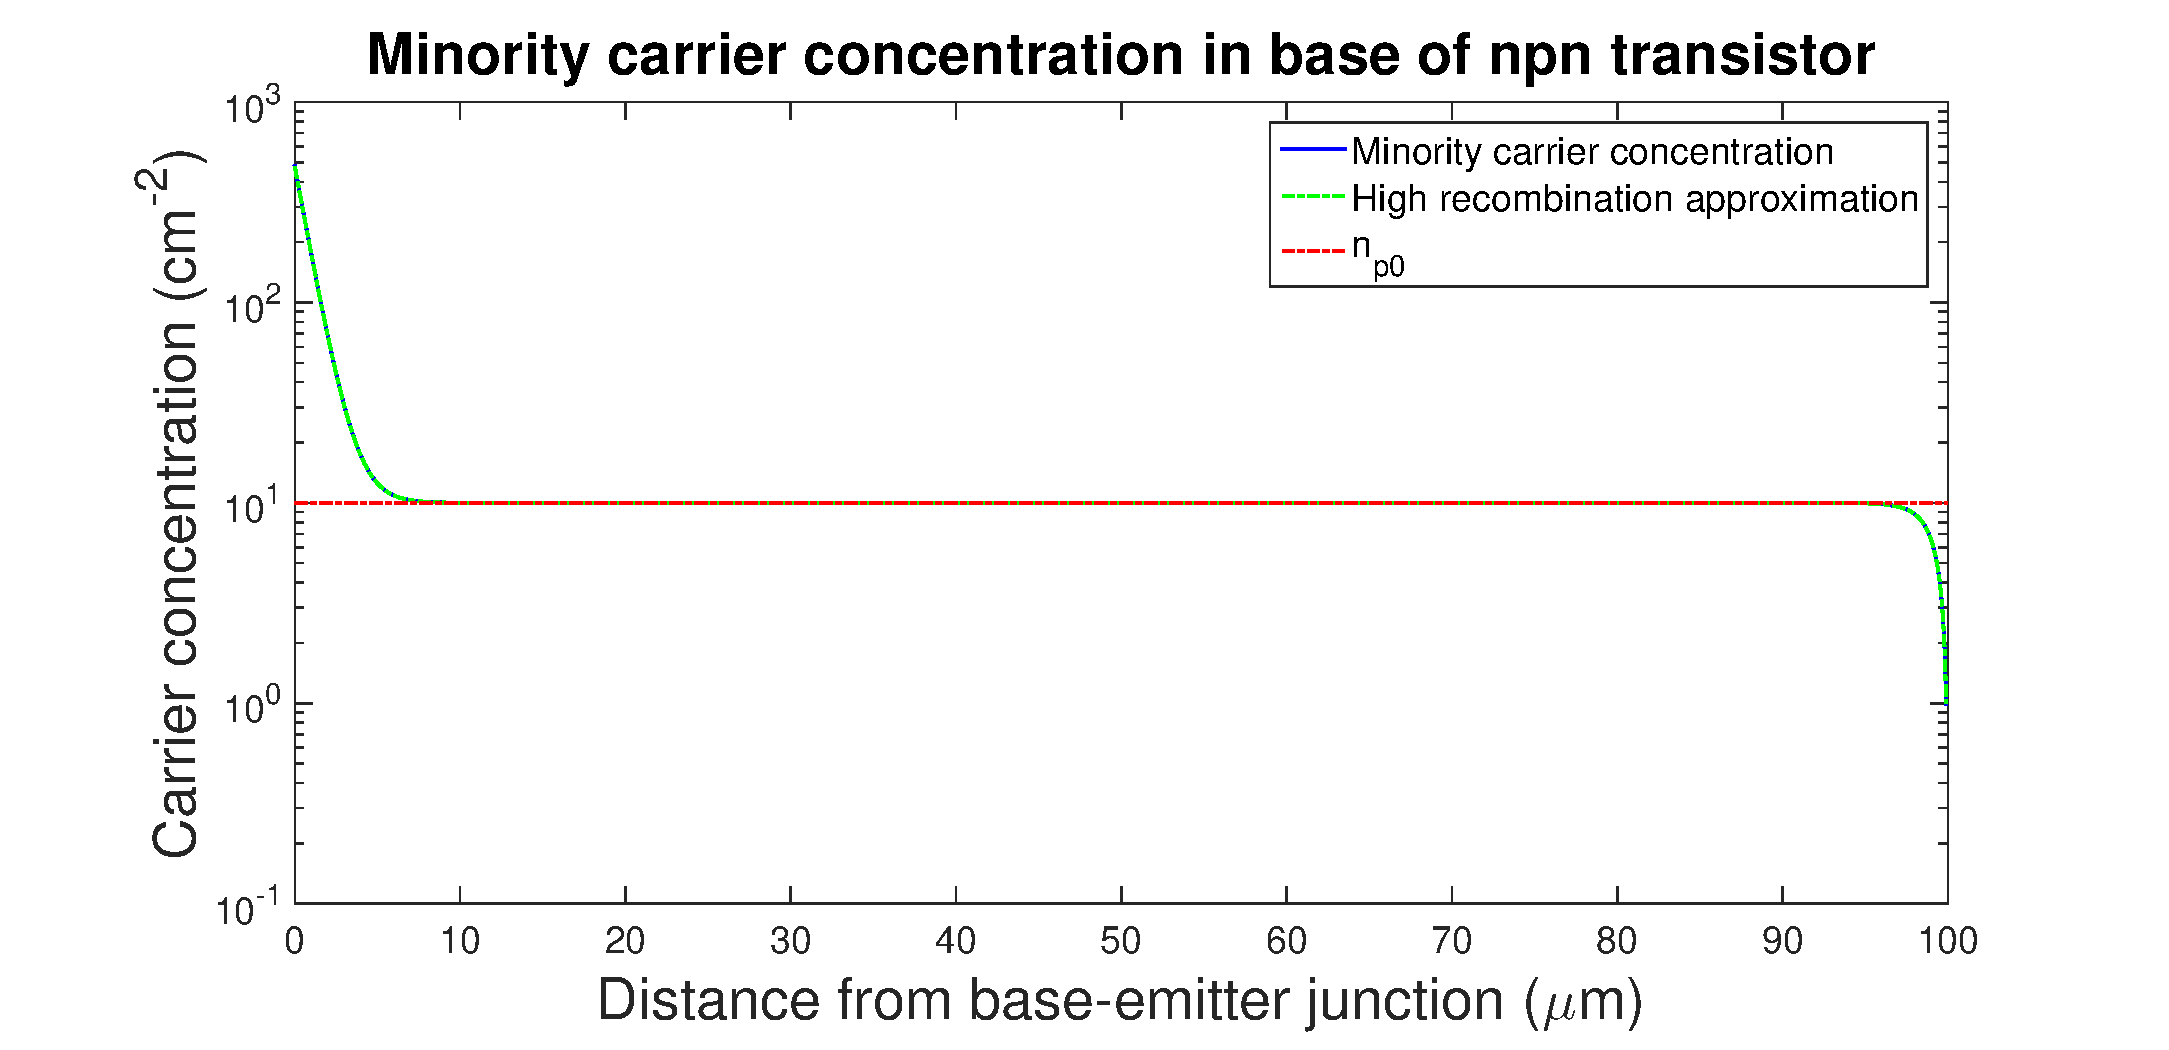
\includegraphics[width=0.8\textwidth]{./img/3d}
		\caption{Minority carrier concentration for a base width $W_B = 100 \mu m$.}
		\label{fig::3d}
	\end{figure}
\subsection*{e)}
	The plot shown in Figure \ref{fig::3e} shows the minority carrier concentration when the base-collector region is slightly forward-biased, and hence the transistor is shuttling carriers from the emitter to the collector, so the npn transistor is operating in the reverse-active region. This aligns with the plot, as the carrier concentration is very steady across the whole base region, remaining above $n_{p0}$ and therefore carriers from the emitter are being ejected from the collector.
	\begin{figure}[htbp!]
		\centering
		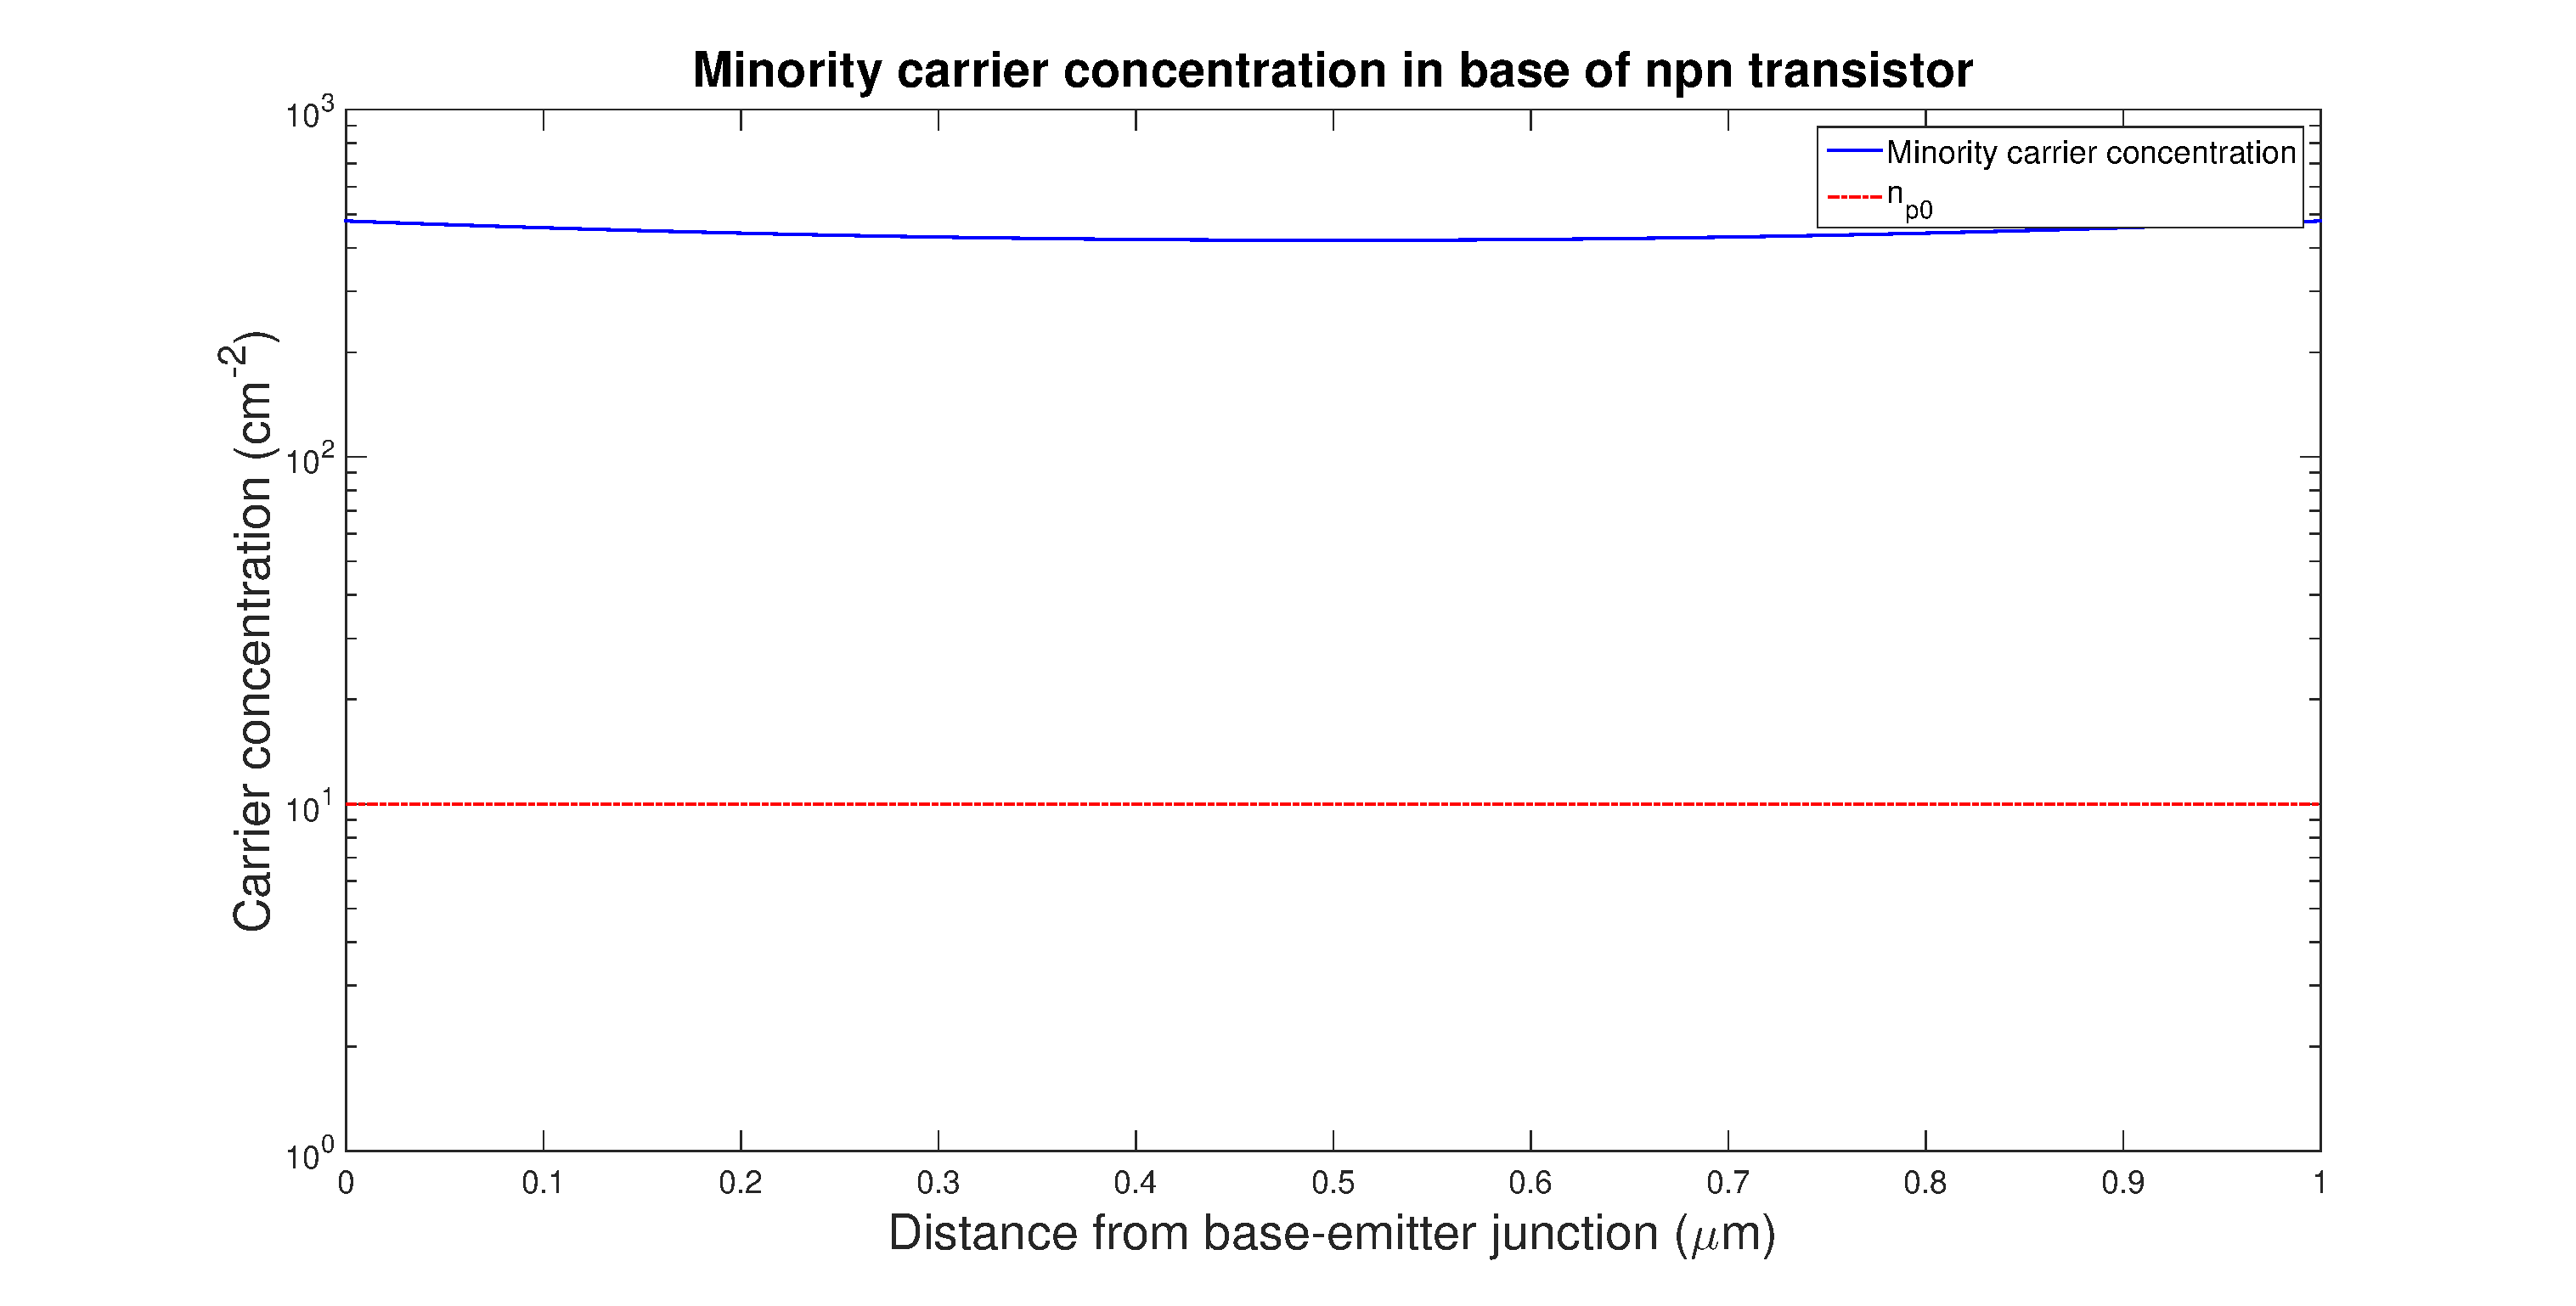
\includegraphics[width=0.8\textwidth]{./img/3e}
		\caption{Minority carrier concentration for a base width $W_B = 1 \mu m$, operating in saturation with $V_{BC} = 0.1 \textrm{ V}$.}
		\label{fig::3e}
	\end{figure}